\documentclass[a4paper]{article}
\usepackage[utf8]{inputenc}
\usepackage{graphicx}

\title{\Large{\textbf{Genetic Algorithm v. 8 Queens}}}
\author{By Robert Bergers}
\date{May 2019}

\begin{document}

\maketitle

% begin abstract
\begin{center}
    \Large{\textbf{Abstract}}
\end{center}
The goal of this project is to create a genetic algorithm that solves the 8 Queens toy problem as fast as possible, and compare the genetic algorithm's performance to a random agent's performance.
% end abstract

\section{Problem}
The 8 Queens problem is a toy problem in which 8 queens have to be placed on a chess board such that no queen can capture another queen. How much faster can a genetic algorithm solve the 8 queens problem on average compared to a random agent?

\section{Hypothesis}
The hypothesis being tested is that a genetic algorithm without the randomness of a random selection method or mutation rate can solve the 8 queens problem at least ten times faster on average than a random agent.

\section{Procedure}

In order to make the problem tractible enough to the point that enough trials could be run to get an accurate estimation of the performance within the given time frame, each row is guaranteed a single queen. The random agent and genetic algorithm only determine the columns in which each queen is placed. The performance of the algorithms are measured in two ways: the mean average of the number of solutions generated by each algorithm before a goal state is found, and the distribution of the performance of each execution of each algorithm. Ten thousand trials of each algorithm have been run, each trial measures the number of solutions generated before a goal state is achieved. \\

\subsection{Random Agent}
The random agent is the control, used as a base with which to compare the performance of the genetic algorithms.\\

\subsubsection{Algorithm}

\begin{itemize}
    \item \textbf{1.} Randomly generate column to place queen in row
    \item \textbf{2.} Repeat step 1 for each row of the board
    \item \textbd{3.} Repeat steps 1-3 until a goal state is achieved
\end{itemize}

\subsection{First Genetic Algorithm}
The first genetic algorithm lightly implements the genetic algorithm paradigm, as in for every 124 generated solutions 100 of them are randomly generated. For both genetic algorithms, the fitness function is $x = c_q_1 + c_q_2 + ... + c_q_8$ where $x$ is the fitness and $c_q$ is the number of queens which each queen is able to capture. The fitness function is to be optimized for the global minimum. \textit{Single-point crossover} and  \textit{best selection} are used for both genetic algorithms as well.\\

\subsubsection{Algorithm}

\begin{itemize}
    \item \textbf{1.} Create and execute 100 random chromosomes
    \item \textbf{2.} Select the best 20\%
    \item \textbf{3.} Splice them randomly
    \item \textbf{4.} Execute 20 spliced chromosomes
    \item \textbf{5.} Get the best 20\%
    \item \textbf{6.} Splice them randomly
    \item \textbf{7.} Execute 4 spliced chromosomes
    \item \textbf{8.} Repeat steps 1-7 until goal state is achieved
\end{itemize}

\subsection{Second Genetic Algorithm}
The second genetic algorithm more heavily emphasizes spliced chromosomes. For every 208 solutions executed by this algorithm, 100 of them are randomly generated.

\subsubsection{Algorithm}

\begin{itemize}
    \item \textbf{1.} Create and execute 100 random chromosomes
    \item \textbf{2.} Get the best 20\%
    \item \textbf{3.} Splice them randomly
    \item \textbf{4.} Execute 20 spliced chromosomes
    \item \textbf{5.} Repeat steps 2 through 4 four times
    \item \textbf{6.} Get the best 20\%
    \item \textbf{7.} Splice them randomly
    \item \textbf{8.} Execute 4 spliced chromosomes
    \item \textbf{9.} Repeat steps 7-8 twice
    \item \textbf{10.} Repeat steps 1-9 until goal state is achieved
\end{itemize}

\section{Results}
The histograms of each algorithm's performance are shown below. The random agent was so much slower than the genetic algorithms that its histogram is on a different scale. Note that for all the histograms, the \textit{x} axis measures the number of solutions generated before a goal state is achieved and the \textit{y} axis measures the number of trials (10,000 trials for each algorithm).
\begin{center}
    \textit{Random agent mean average solutions}: 182,556\\
    \textit{First genetic algorithm mean average solutions}: 75,848\\
    \textit{Second genetic algorithm mean average solutions}: 48,936\\
\end{center}
\begin{figure}[h!]
\begin{subfigure}
    \centering
        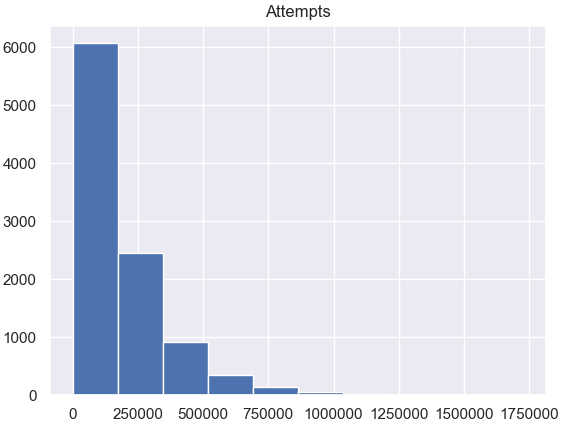
\includegraphics[width=0.8\columnwidth]{random_agent.png}
        \caption{Random agent performance distribution}
        \label{ra}
\end{subfigure}
\begin{subfigure}
    \centering
        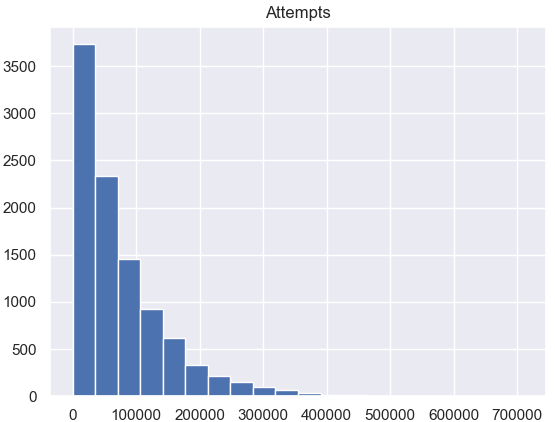
\includegraphics[width=0.8\columnwidth]{ga_trial_one.png}
        \caption{GA trial 1 performance distribution}
        \label{ga1}
\end{subfigure}
\begin{subfigure}{\linewidth}
    \centering
        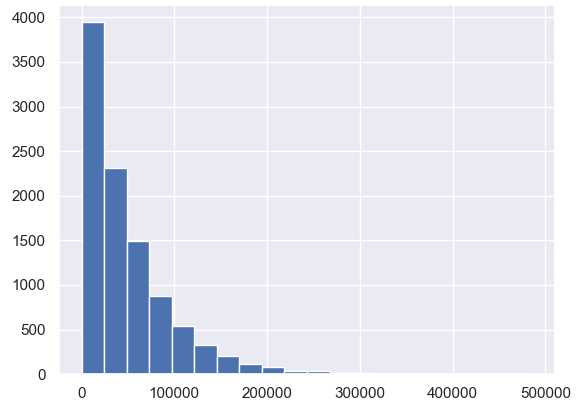
\includegraphics[width=0.8\linewidth]{ga_trial_two.png}
        \caption{GA trial 2 performance distribution}
        \label{ga2}
\end{subfigure}
\end{figure}
\section{Conclusion}
While both genetic algorithms were substantially more successful than the random agent, the hypothesis that a genetic algorithm could run 10 times faster on average could not be proven.\\

It would make sense initially that a third genetic algorithm which spliced the random population even more could reach the expected 10x average performance, however this is likely not the case. The first genetic algorithm was around 20\% different from the random agent (124/24 = 19\% of the chromosomes were spliced by the algorithm), yet had an average speed that was around 2.4 times faster than the random agent. The second genetic algorithm spliced chromosomes almost 5 times more than the first (24/108 = 22\%), it only ran around 3.7 times faster than the random agent. Since the second algorithm was less than twice as efficient on average than the first, yet spliced almost 5 times as many chromosomes, this method of selection and crossover likely yields diminishing returns.\\

This is not to say, however, that it is impossible for a genetic algorithm to perform 10 times better than a random agent. Due to the nature of this experiment, the results can either prove that a genetic algorithm can run 10 times faster or the results can be inconclusive. It is still possible that there is a better crossover or selection process could solve the 8 queens problem with the expected efficiency. It is also possible that a mutation probability, which was ommitted from both genetic algorithms, could make the genetic algorithm more efficient.
\end{document}
